%----------------------------------------------------------------------------
\chapter{Sensors}
\label{chap:sensors}
%----------------------------------------------------------------------------

Selecting the right sensors to understand the environment is half the task.
Combining multiple sensors to collect data for further information extraction is
called sensor fusion. In this chapter we are going to detail the most widely
used sensors for scene understanding for autonomous vehicles and compare them. 

Radar, utrasonic and LiDar sensors basically all work the same: emit a wave,
wait until it returns and estimate the distance based on the time difference,
and estimate the speed calculating the frequency shift - this is the Doppler
effect: an increase in frequency corresponds to an object approaching and vice
versa. A visualization is seen on \refstruc{fig:sensors}.

\begin{figure}[!ht]
    \centering
    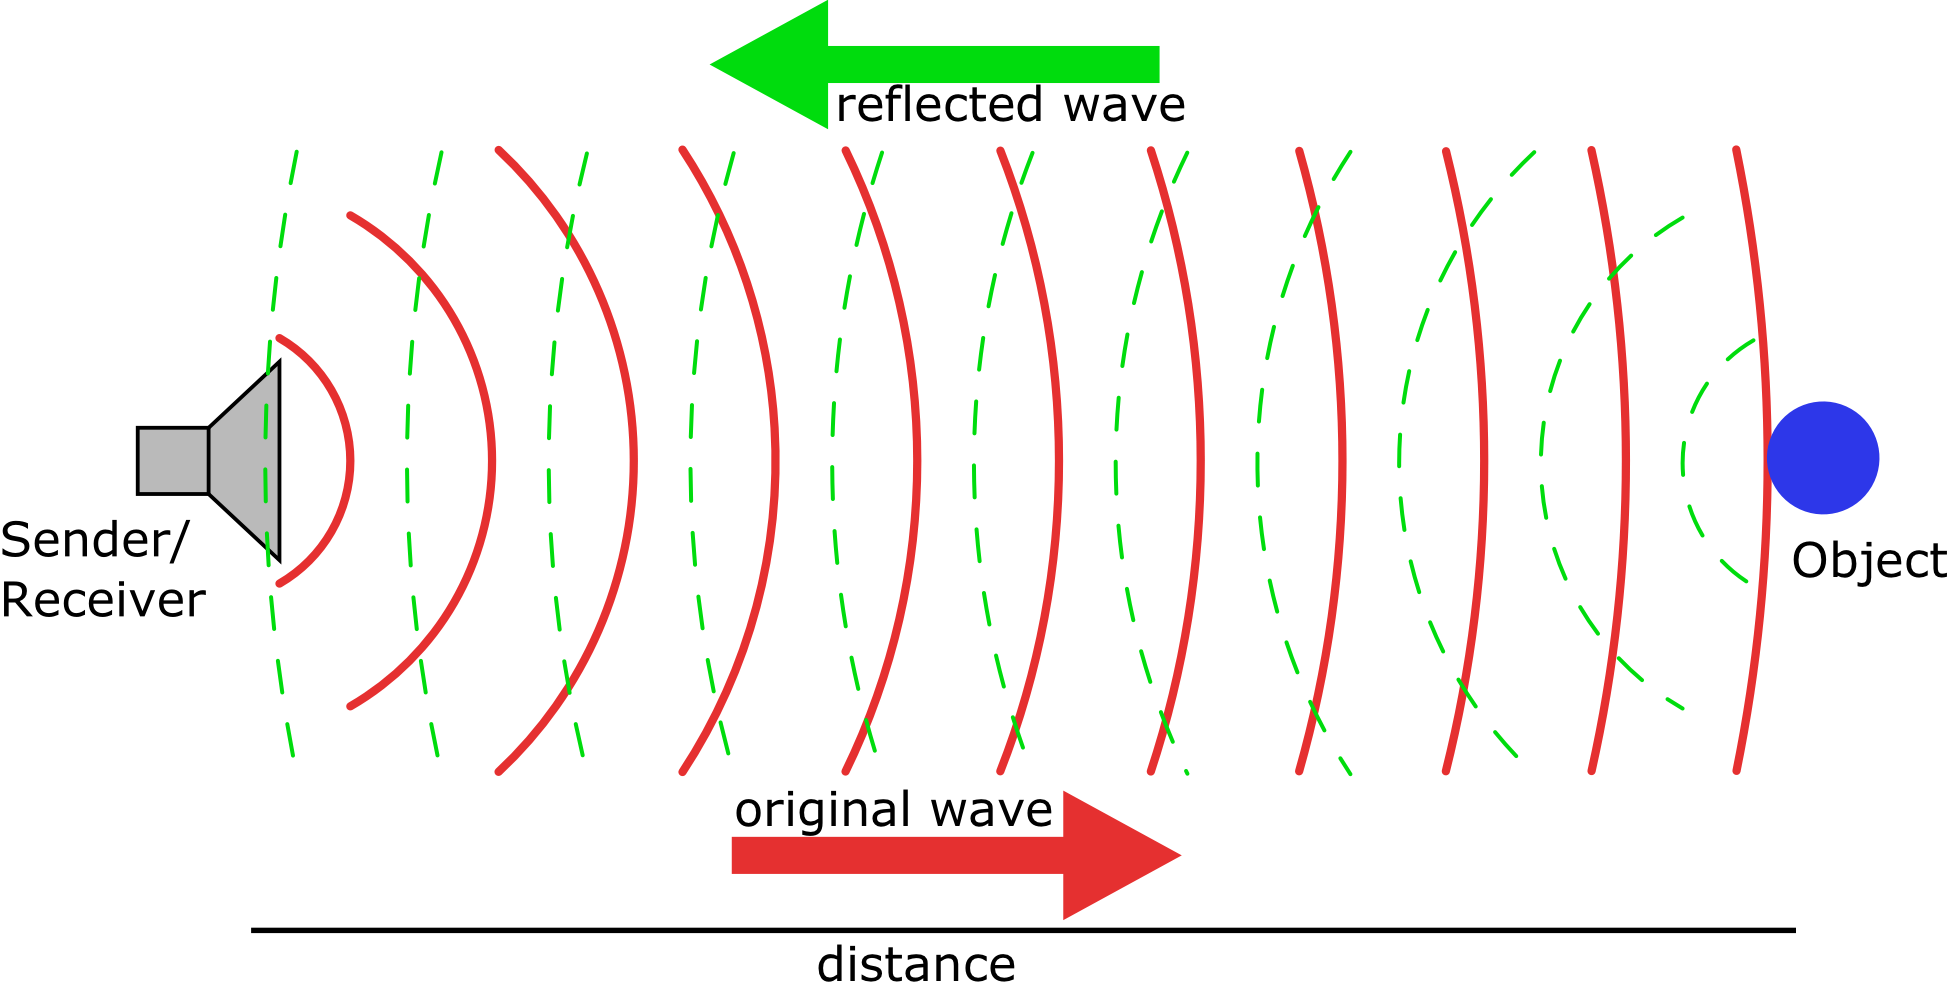
\includegraphics[width=150mm, keepaspectratio]{figures/sensors.png}
    \caption{Sensing object with wave emission and reflection}
    \label{fig:sensors}
\end{figure}

Thus calculating the distance is a simple equation:

\begin{align}
Distance=\frac{Speed\; of\; wavefrom * Time\; of\; Flight}{2}
\end{align}

However they use different waves: Radar works with electromagnetic waves,
ultrasonic sensors work with sound waves and LiDar works with laser light.

\section{Radar}

Radar sensors at the front, rear and sides have become an essential component in
modern production vehicles. Though most frequently used as part of features like
parking assistance and blind-spot detection, they have the capability to detect
objects at much greater range – several hundred meters in fact.

Radar sensors are excellent at detecting objects, but they’re also excellent for
backing up other sensors. For instance, a front-facing camera can’t see through
heavy weather. On the other hand, radar sensors can easily penetrate fog and
snow, and can alert a driver about conditions obscured by poor conditions. Radar
is robust in harsh environments (bad light, bad weather, extreme temperatures).

Automotive radar sensors can be divided into two categories: short-range radar
(SRR), and long-range radar (LRR). The combination of these types of radar
provides valuable data for advanced driver assistance systems.

\textbf{Short-range radar (SRR)}
Short-range radar (SRR): Short-range radars (SRR) use the 24 GHz frequency and
are used for short range applications like blind-spot detection, parking aid or
obstacle detection and collision avoidance. These radars need a steerable
antenna with a large scanning angle, creating a wide field of view. 


\textbf{Long-range radar (LRR)}
Long-range radar (LRR): Long-range radars (LRR) using the 77 GHz band (from
76-81GHz) provide better accuracy and better resolution in a smaller package.
They are used for measuring the distance to, speed of other vehicles and
detecting objects within a wider field of view e.g. for cross traffic alert
systems. Long range applications need directive antennas that provide a higher
resolution within a more limited scanning range. Long-range radar (LRR) systems
provide ranges of 80 m to 200 m or greater.

\section{Ultrasonic}

Ultrasonic (or sonar) sensors like radar, can detect objects in the space around
the car. Ultrasonic sensors are much more inexpensive than radar sensors, but
have a limited effective range of detection. Because they’re effective at short
range, sonar sensors are frequently used for parking assistance features and
anti-collision safety systems. Ultrasonic sensors are also used in robotic
obstacle detection systems, as well as manufacturing technology. In comparison
to infrared sensors in proximity sensing applications, ultrasonic sensors are
not as susceptible to interference of smoke, gas, and other airborne particles
(though the physical components are still affected by variables such as heat),
and they are independent of light conditions. They also work based on reflected
emission. 

Ultrasound signals refer to those above the human hearing range, roughly from 30
to 480 kHz. For ultrasonic sensing, the most widely used range is 40 to 70 kHz.
At 58 kHz, a commonly used frequency, the measurement resolution is one
centimeter, and range is up to 11 meters. At 300 kHz, the resolution can be as
low as one millimeter; however, range suffers at this frequency with a maximum
of about 30 cm.

You can see the sensor suite of Tesla \refstruc{fig:teslasensors} from
Tesla Autopilot website \footnote{Tesla autopilot
\url{https://www.tesla.com/autopilot}}.

\begin{figure}[!ht]
    \centering
    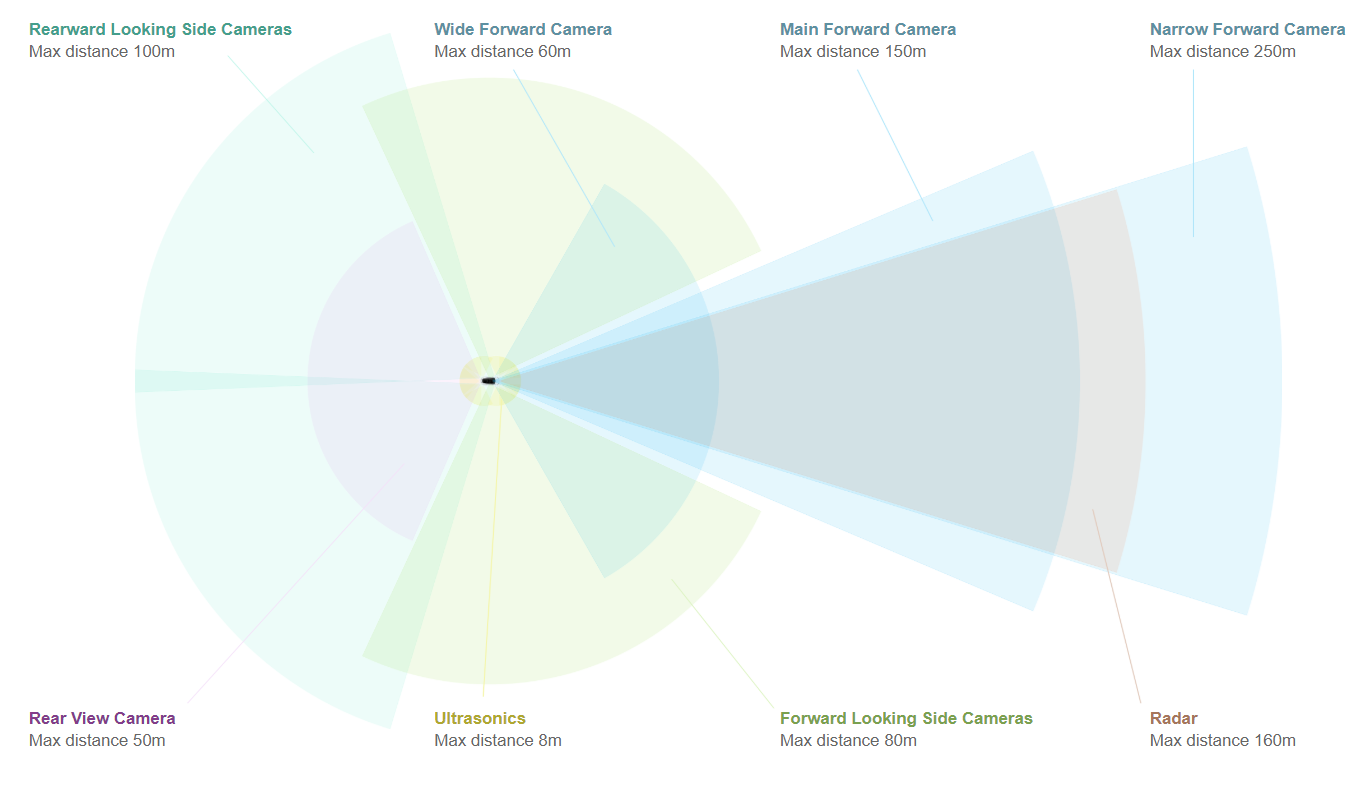
\includegraphics[width=150mm, keepaspectratio]{figures/teslasensors.png}
    \caption{Tesla sensor suite infographic }
    \label{fig:teslasensors}
\end{figure}


\section{LiDAR}

As Radar is to radio waves, and sonar is to sound, LiDAR (Light Detection and
Ranging) uses lasers to determine distance to objects. Lidar sometimes is called
3D laser scanning. It does this by spinning a laser across its field of view and
measuring the individual distances to each point that the laser detects. This
creates an extremely accurate (within 2 centimeters) 3D scan of the world around
the car.

The principle behind LiDAR is really quite simple. Shine a small light at a
surface and measure the time difference it takes to return to its source. The
equipment required to measure this needs to operate extremely fast. The LiDAR
instrument fires rapid pulses of laser light at a surface, some at up to 150,000
pulses per second. A sensor on the instrument measures the amount of time it
takes for each pulse to bounce back. Light moves at a constant and known speed
so the LiDAR instrument can calculate the distance between itself and the target
with high accuracy. By repeating this in quick succession the insturment builds
up a complex 'map' of the surface it is measuring.

The three most common currently used or explored wavelengths for automotive
lidar are 905 nm, 940 nm and 1550 nm, each with its own advantages and
drawbacks.

Lidar sensors are able to paint a detailed 3D point cloud of their environment
from the signals that bounce back instantaneously. It provides shape and depth
to surrounding cars and pedestrians as well as the road geography. And, like
radar, it works just as well in low-light conditions.

You can see how a lidar sensor from Luminar\footnote{Luminar
\url{https://www.luminartech.com/}} reconstructs the environment in
\refstruc{fig:luminar}.

\begin{figure}[!ht]
    \centering
    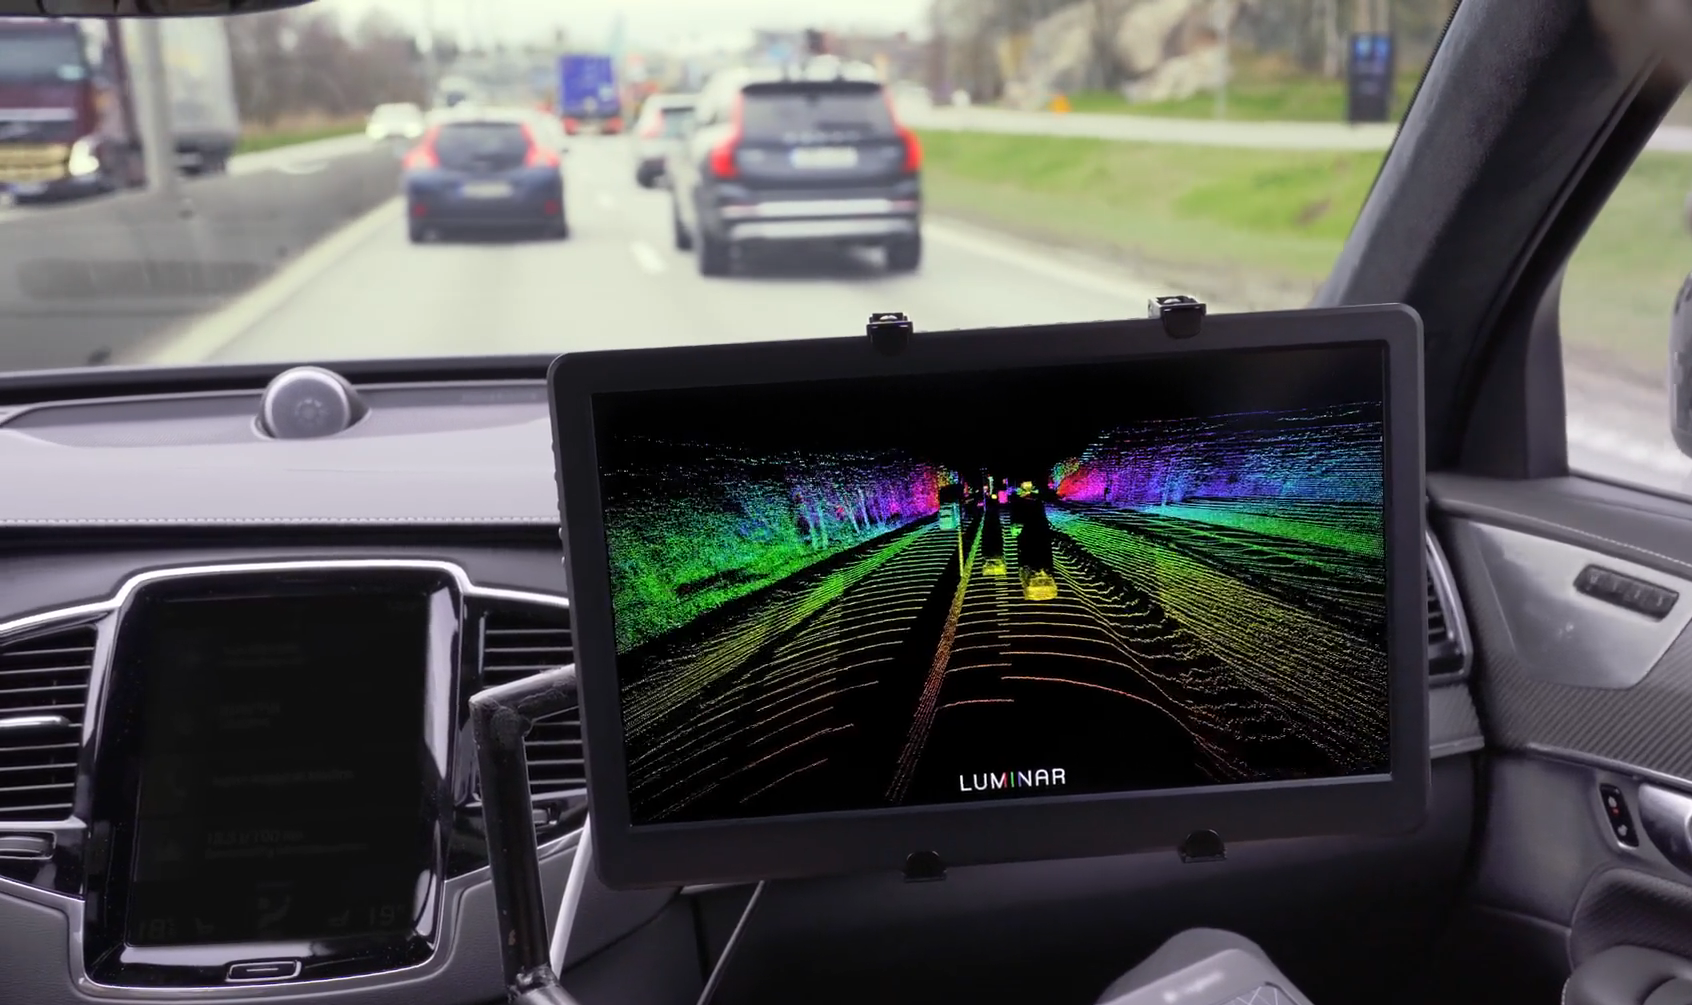
\includegraphics[width=150mm, keepaspectratio]{figures/luminar.png}
    \caption{Luminar LiDAR in action}
    \label{fig:luminar}
\end{figure}


Currently, LiDAR units are very big, and fairly expensive - as much as 10 times
the cost of camera and radar — and have a more limited range. You will most
often see them mounted on Mapping Vehicles, but as the technology becomes
cheaper, we might see them on trucks and high-end cars in the near future.

\section{RGB Cameras}

Cameras are the essential sensors for self-driving cars. Most imaging sensors
are sensitive from about 350 nm to 1000 nm wavelengths. The most common types of
sensors for cameras are CCD (charged coupled device) and CMOS (complementary
metal–oxide–semiconductor). The main difference between CCD and CMOS is how they
transfer the charge out of the pixel and into the camera’s electronics.

CCD-based image sensors currently offer the best available image quality, and
are capable of high resolutionsm making them the prevalent technology for still
cameras and camcorders.

An important aspect of cameras is the camera model that describes how points of
the world translate to pixels in the image. That is going to be essential when
we want to apply the inverse projection to determine the world-position of
objects in the picture. I will talk about this in the next chapter. 


\section{GPS \& WPS}

The Global Positioning System is the perfect example of how sensor
technology grows smaller and more ubiquitous over time. Originally introduced
for military applications in 1974, GPS probes today can be found in cameras,
watches, key fobs, and of course, the smartphone in your pocket.

The lesser-known WPS stands for Wi-Fi Positioning System, which operates
similarly. When a probe detects satellites (GPS) or Wi-Fi networks (WPS), it can
determine the distance between itself and each of those items to render a
latitude and longitude. The more devices a GPS/WPS probe can detect, the more
accurate the results. On average, GPS is only accurate to around 20 meters.

For WPS the most common and widespread localization technique is based on
measuring the intensity of the received signal, and the method of
"fingerprinting". Typical parameters useful to geolocate the wireless access
point include its SSID and MAC address. The accuracy depends on the number of
nearby access points whose positions have been entered into the database. The
Wi-Fi hotspot database gets filled by correlating mobile device GPS location
data with Wi-Fi hotspot MAC addresses.